%%%%%%%%%%%%%%%%%%%%%%%%%%  phdsymp_sample2e.tex %%%%%%%%%%%%%%%%%%%%%%%%%%%%%%
%% changes for phdsymp.cls marked with !PN
%% except all occ. of phdsymp.sty changed phdsymp.cls
%%%%%%%%%%                                                       %%%%%%%%%%%%%
%%%%%%%%%%    More information: see the header of phdsymp.cls   %%%%%%%%%%%%%
%%%%%%%%%%                                                       %%%%%%%%%%%%%
%%%%%%%%%%%%%%%%%%%%%%%%%%%%%%%%%%%%%%%%%%%%%%%%%%%%%%%%%%%%%%%%%%%%%%%%%%%%%%%


%\documentclass[10pt]{phdsymp} %!PN
\documentclass[twocolumn]{phdsymp} %!PN
%\documentclass[12pt,draft]{phdsymp} %!PN
%\documentstyle[twocolumn]{phdsymp}
%\documentstyle[12pt,twoside,draft]{phdsymp}
%\documentstyle[9pt,twocolumn,technote,twoside]{phdsymp}

\usepackage[english]{babel}       % Voor nederlandstalige hyphenatie (woordsplitsing)

\usepackage{graphicx}                   % Om figuren te kunnen verwerken
\usepackage{graphics}			% Om figuren te verwerken.
\graphicspath{{figuren/}}               % De plaats waar latex zijn figuren gaat halen.

\usepackage{times}


\hyphenation{si-mu-la-ted re-a-lis-tic packets really in-clu-ding}

%\def\BibTeX{{\rm B\kern-.05em{\sc i\kern-.025em b}\kern-.08em
%    T\kern-.1667em\lower.7ex\hbox{E}\kern-.125emX}}
\bibliographystyle{phdsymp}
\newtheorem{theorem}{Theorem}

\begin{document}

\title{One-shot learning of gestures using a convolutional neural network} %!PN

\author{Jasper Vaneessen}

\supervisor{Lionel Pigou}


\maketitle

\begin{abstract}
A lot of research has been done in the field of sign language recognition, in order to aid in the communication between the deaf and hearing communities.  One of the most promising techniques for an automatic recognition system is that of convolutional neural networks (CNN). This kind of self-learning feature-extractor, paired with a classification algorithm such as an artificial neural network (ANN), achieves highly competitive results on several recognition tasks. The downside is that they require a lot of data to achieve these results.

Sign language, just as any other language, changes frequently. Every year new gestures are added to the lexicon of a language. If a predictive model has to learn to recognize these new gestures, it requires a lot of training examples of these new gestures and a full retraining of the model. This study tries to expand the recognizable lexicon of a CNN-based gesture recognition system, using only a few examples and minimum retraining. It does this by adding new softmax units to an existing model and only retraining the weights of these new units. This way the features the CNN has learned to detect from previous knowledge are kept and re-used to categorize the new gesture. It is shown that using this method it is possible to add multiple gestures subsequently, yielding a dynamically expandable recognition system.
\end{abstract}

\begin{keywords}
One-shot learning, convolutional neural networks, gesture recognition, ChaLearn LAP 2014
\end{keywords}

\section{Introduction}
Sign language is the main form of communication in the deaf and hard-of-hearing community. It is a highly visual-spatial, linguistically complete and natural language. Instead of using acoustically conveyed sound patterns, sign language combines hand shapes, orientation and location as well as movement of arms and body \cite{buyens_gebarentaaltolken_2003}.
\par When deaf people want to convey a message to non-signing people, they have to rely on interpreters or text writing. Interpreters can be very expensive and their availability is limited, while writing down everything you want to say can be very inconvenient. Furthermore, sign language is not at all universal. Different countries have different sign languages and some even have regional ones \cite{VGT-standard}. Thus, even proficiency in a certain sign language does not guarantee the ability to communicate with all deaf people.
\par The field of automatic sign language recognition tries to solve some of these issues. The use of convolutional neural networks (CNN's) has proven to be very succesful in various recognition tasks including gesture recognition as described in \cite{wu_deep_2014}, \cite{cnn-ji} and \cite{lionel}. CNN's are deep learning models that can be viewed as self-learning feature extractors. By feeding them examples, they learn to extract certain features from an image, which can then be used by a classification model, such as an artificial neural network (ANN), to make predictions.
\par A sign language, just as any other natural language, is prone to change over time. A functional gesture recognition system will have to account for this possibility of lexicon expansion. To expand a CNN with a new gesture, it would have to be retrained completely with a large number of examples of this gesture. Gathering all these examples will take a lot of time and effort. The complete retraining of a CNN will also take up a lot of processing time.
\par This work proposes a system to expand the recognizable lexicon of a gesture recognition system based on a CNN. Key challenges in this endeavour are the use of a limited amount of samples and retraining as little of the network as possible. Ideally, the model would need only one sample to learn and distinguish a new gesture. The influence of the number of used samples is examined with the end-goal of learning from one example. This is called one-shot learning.

%\section{Related work}

\section{Methodology}
\subsection{Dataset and input}
To train the CNN we need a lot of data. The dataset used here is the one made available for the \textit{ChaLearn Looking at People 2014 Track 3: Gesture Spotting} (CLAP14) challenge (\cite{escalera_chalearn_2014}). This dataset consists of 20 gestures from Italian culture, performed by 27 users, with variations in background, lighting, clothing and physique. The gestures are captured using a Microsoft Kinect \cite{kuhn2011kinect} so that each image has four seperate streams: RGB-image, depth-image, joint positions (skeleton-map) and user index (location of user in depth map).

There are ten thousand samples available in total. These are divided into three sets: six thousand for the training set and two thousand each for the validation- and test set. The users in the dataset appear alphabetically and the three sets are divided sequentially, meaning there is some user-overlap between training- and validation set but no overlap between, training- and test set.

For each gesture, a pre-processing step is used from \cite{lionel}: both hands are tracked and cropped into a seperate datastream. The images of the two hands and upper body are scaled and cropped to a size of 64x64 pixels. Only the depth image is used, since in both \cite{wu_deep_2014} and \cite{lionel} these delivered the best performance. For each gesture four frames are extracted, leaving an input of 12x64x64 that will be used for gesture recognition.
\begin{figure*}
	\def\svgwidth{\textwidth}
	\input{figuren/First-model.pdf_tex}
	\caption{Architecture of the basemodel, consisting of three convolutional layers, two hidden layers and a softmaxlayer with twenty output units.}\label{fig:model}
\end{figure*}
\subsection{Convolutional neural network}
The idea of CNN's stems from research on the visual cortex of respectively a cat and a monkey in \cite{hubel1968receptive}. The cortex consists of simple and complex cells. The simple cells perform the feature extraction while the complex cells combine local features from a small spatial neighborhood. This is called spatial pooling and it is crucial to obtain a translation-invariant result.

Convolutional Neural Networks (CNN) try and mimic this principle. Their use in state-of-the-art applications such as \cite{cnn-karpathy} and \cite{krizhevsky2012imagenet} confirm their advantages. CNN's consist of alternating convolutional and pooling layers. The convolutional layer functions as a feature extractor with several feature maps in each layer. Each feature map detects another feature and the amount of feature maps per layer increases the deeper we go into the network. Pooling layers combine these features to a smaller resolution, thus ensuring a translation invariant detection.

The network learns from examples as humans do. It looks at an example, tries to predict the gesture and checks its result with the actual gesture. If it is wrong, the network learns from its mistakes and adjusts itself. Thus all we have to do is let our network learn from a big set of examples and optimize this learning process.
In the case of one-shot learning and expanding the recognizable lexicon, the features already learned from a big dataset of gestures will be used to classify the new gesture. This is done by only retraining the top layers of the network, which combine the different feature detections and thus make a prediction.
\subsection{Baseline model for all gestures}
First, a baseline model is constructed. This model is then optimized for the task of recognizing all twenty gestures from the CLAP 2014 dataset. The architecture and hyperparameters from this baseline model are then used in the one-shot learning experiments. Figure \ref{fig:model} shows the architecture of this predictive model. 

Feature-extraction is done by a CNN of three layers and classification is done by an ANN with two hidden layers and one softmax layer which outputs the class-wise predictions. All artificial neurons are rectified linear units (ReLUs as seen in \cite{ReLU} and \cite{wu_deep_2016}).

To regularize the model dropout is performed during the training phase (\cite{dropout}). Data-augmentation is also performed, all samples are scaled, rotated and translated by a small amount on the CPU while the GPU is used for the training of the predictive model.

For training, Nesterov's accelerated gradient (NAG, \cite{botev_nesterovs_2016} and \cite{sutskever2013importance}) is used with a mini-batch size of 32 and momentum-coefficient of 0.9. The learning rate is fixed at $10^{-4}$, all the weights are initialized using Xavier initialization as described in \cite{glorot-1} and all biases are set to 0.

The programming environment used is Python, the models are implemented by using the open Python libraries Theano \cite{theano}, and Lasagne \cite{lasagne}. Theano enables easy use of GPU-acceleration. All the training is performed on computers of the Reservoir Labs at the Department of Electronics and Information Systems of UGent. These have hexacore processors (Intel Core i7-3930K) and NVIDIA Tesla K40c graphics cards.

This model achieves an overall accuracy of 81.20\% on the classification of the 2000 gestures from the test set. The precision and recall values of each gesture are used as a baseline for future experiments.
\section{Experiments and results}
Several experiments are set up to test the expandability of the predictive model. One gesture is excluded from the dataset and this subset is then used to train the predictive model. This model is trained until convergence after which it can be retrained with the excluding training set plus some examples of the new gesture. Two of these experiments will be discussed here.

\subsection{Softmax19+1 model}
\begin{figure}
	\centering
	\def\svgwidth{0.6\columnwidth}
	\input{figuren/softmax19+1.pdf_tex}
	\caption{Architecture of the softmax19+1 model. Only the yellow weights of the new unit are retrained.}\label{fig:19x1-model}
\end{figure}
A model equal to that of the baseline model is used with only one difference: the final softmaxlayer (as seen in Figure \ref{fig:19x1-model}). The pretrained model has a softmax layer of nineteen units for the classification of nineteen gestures. After pretraining, the model is expanded with one extra unit, also fully connected to the dense layer with one hundred units. To keep all functionality on the classification of the nineteen already learned gestures, only the weights of the new softmax unit are trained.

\begin{figure}
	\def\svgwidth{\columnwidth}
	\input{figuren/19x1-oneshot-vgl.pdf_tex}
	\caption{Precision and recall values of the softmax19+1 model when retraining with 1 and 10 samples. The precision and recall scores of the baseline model are plotted as well for comparison.}\label{fig:19x1}
\end{figure}

For each gesture in the dataset a model is trained, excluding this gesture from training. Afterwards this model is retrained with one sample and with ten samples of the new gesture. Training is stopped when the loss on the validation set (which includes all samples of the new gesture) has stopped declining for some iterations. In Figure \ref{fig:19x1} the results of this experiment are shown, together with the baseline results of the given gestures. Precision and recall values of the softmax19+1 model both follow the same trend as those of the baseline model. Recall scores are mostly dependent on the amount of samples used.
In experiments where gesture 14 and 15 were retrained several times with varying amounts of samples (from one sample to two hundred), it is notable that the recall score climbs the steepest between the use of one to ten samples. After using more than ten samples, the curve flattens, meaning use of more data does not help performance as much.

\subsection{Softmax18+1+1 model}
\begin{figure}
	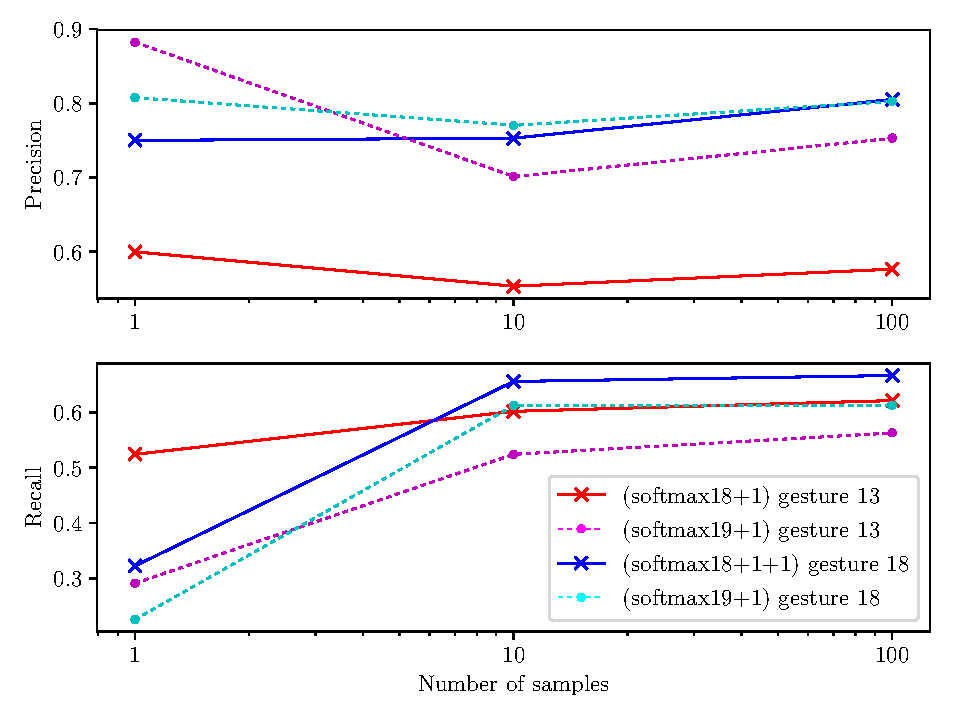
\includegraphics[width=\columnwidth]{18x2.pdf}
	\caption{Precision and recall values of the softmax18+1+1 model. Gesture 13 is learned first (softmax18+1) followed by gesture 18 (softmax18+1+1). The dashed lines present a comparison to the performance of the softmax19+1 model on the same gestures.}\label{fig:18x2}
\end{figure}
The final experiment is that of the so-called \textit{softmax18+1+1} model. In this model two gestures are learned subsequently. First a model with a softmaxlayer of eightteen units is trained. Then the model is expanded with one extra softmax unit for the new gesture, just as in the softmax19+1 model. When the first gesture is learned, the model is expanded again with another softmax unit for a second gesture.

Figure \ref{fig:18x2} shows the results of a variation of  this experiment where gesture 13 is learned first and gesture 18 is learned afterwards. The precision and recall values of this model are plotted against the values of the softmax19+1 model. The recall scores of the softmax18+1+1 model not only match the ones of the softmax19+1 model, they are higher. These results clearly show that the used method provides a way to dynamically add multiple gestures to a pretrained model, without loss of performance.


\section{Conclusion}
The results of this study show that there is great potential for expanding the recognizable lexicon of a CNN using only a few examples and only retraining a small amount of parameters. The gap between learning with one, few or all samples is still apparent, but a more complex model, the use of extra preprocessing steps and more advanced methods of data-augmentation can surely help close this gap.

After using more than ten samples, the gain in performance flattens significantly. The region between the use of one to ten samples is an interesting region for further investigation.

The method of dynamically adding a unit for each new gesture and only training the weights of this unit shows to be quite effective, even when adding multiple gestures subsequently. Using this method it is possible to keep adding gestures to a model, given it has acquired enough generalized knowledge from its pretraining on a larger dataset.




\nocite{*}
\bibliography{bibliodatabase}
\end{document}

%%%%%%%%%%%%%%%%%%%%%  End of phdsymp_sample2e.tex  %%%%%%%%%%%%%%%%%%%%%%%%%%%
